\documentclass[12]{article}
\usepackage{tikz}
\usetikzlibrary{positioning}
\definecolor{processblue}{cmyk}{0.96, 0, 0, 0}
\usepackage{import}
\usepackage{transparent}
\usepackage{xcolor}
\usepackage{tcolorbox}
\usepackage{amsmath}
\usepackage{upgreek}
\usepackage{enumitem}
\usepackage{amssymb}
\usepackage[margin=0.25in]{geometry}
\usepackage{listings}
\usepackage[T1]{fontenc}
%\geometry{letterpaper}
%Commands definitions
\newcommand{\setbackgroundcolour}{\pagecolor[rgb]{0.19, 0.19, 0.19}}
\newcommand{\settextcolour}{\color[rgb]{0.87, 0.87, 0.87}}
\newcommand{\invertbackgroundtext}{\setbackgroundcolour\settextcolour}

%Command execution
%If this line is commented, then the appearance remaind as usual.
\invertbackgroundtext

\lstset{
    language=C,
    basicstyle=\ttfamily,
    keywordstyle=\color{cyan},
    commentstyle=\color{green!70!black},
    stringstyle=\color{red},
    showstringspaces=false,
    tabsize=4,
    breaklines=true,
    breakatwhitespace=false,
}

% Ponizsze linijki sa templatka do zadan i problemow                                                                                                           
% Wziete gdzies z internetu
% Assignment class for homework and exams.                                                                                                                  
%
% Gabriel Antonius
%
%
\NeedsTeXFormat{LaTeX2e}
\RequirePackage{placeins}
\RequirePackage{environ}
\RequirePackage{xifthen}


% \solutiontrue and \solutionfalse control whether solutions are shown
\newif\ifsolution
\solutiontrue
%\solutionfalse


% Redefine these if you want to change the language
\newcommand{\problemlabel}{Zadanie}
\newcommand{\solutionlabel}{Rozwi\k{a}zanie}


% Set up counters for problems and subproblems
\newcounter{ProblemNum}
\newcounter{SubProblemNum}[ProblemNum]
\renewcommand{\theProblemNum}{\arabic{ProblemNum}}
\renewcommand{\theSubProblemNum}{\alph{SubProblemNum}}


% The problem environment is the base unit of content for this class.
\newcommand{\subsectiontitle}{}
\newenvironment{problem}[1]%
  {
  \stepcounter{ProblemNum}
  \renewcommand{\subsectiontitle}{\problemlabel \ \theProblemNum \ifthenelse{\isempty{#1}}{}{: #1}}
  \medskip \subsection*{\subsectiontitle}  % new line after title
  {\large Tre\'{s}\'{c}: } 
  \FloatBarrier
  }
  {
  \FloatBarrier
  }


% The subproblem command divides a problem into parts a), b), c), ...
\newcommand*{\subproblem}{%
  \vspace*{3pt}
  \stepcounter{SubProblemNum}%
  {\bf \theSubProblemNum)\hspace{2pt}}
  }


% The solution environment should be used within the problem environment
\NewEnviron{solution}{
  \setcounter{SubProblemNum}{0}
  \ifsolution
    \FloatBarrier
    \subsubsection*{\solutionlabel}
    \BODY
  \fi}


%\documentclass[12pt]{myassignment}
%\usepackage{amsmath}                                                                                                                                        
\setlength{\parindent}{0pt}

\solutiontrue  % <---- Toggle showing solutions or not
%\solutionfalse

%koniec templatki do zadan i problemow




%\author{Lukasz Kopyto}
%\title{tytul}

\begin{document}
%\maketitle
\noindent \L ukasz Kopyto \hfill 07.12.2024 \\

\begin{center}

    {\large Tresc i rozwiazania listy numer 9 z Matematyki Dyskretnej(M)}
\end{center}

\begin{problem}{Problem przewoznika}
        
    Przewoznikowo polecono przewiezc przez rzeke wilka, koze i kosz z kapusta. Oprocz przewodnika, lodka moze pomiescic tylko jeden z tych trzech przedmiotow. Jak musi postapic przewoznik, jesli nie moze pozostawic samych na brzegu wilka z koza i kozy z kapusta? Narysuj graf ilustrujacy rozwiazanie tego problemu.


\begin{solution}

    Niech A to bedzie koza, B to Wilk oraz C to kapusta. Wierzcholek niebieski oznacza brzeg, na ktorym pierwotnie znajduja sie koza, wilk i kapusta, a wierzcholek czerwony oznacza brzeg docelowy. Przykladowo: jesli jestesmy w wierzcholku niebieskim z oznaczeniem AC, to znaczy to, ze jestesmy na brzegu pierwszym/startowym razem z koza oraz kapusta.
\begin{center}
    
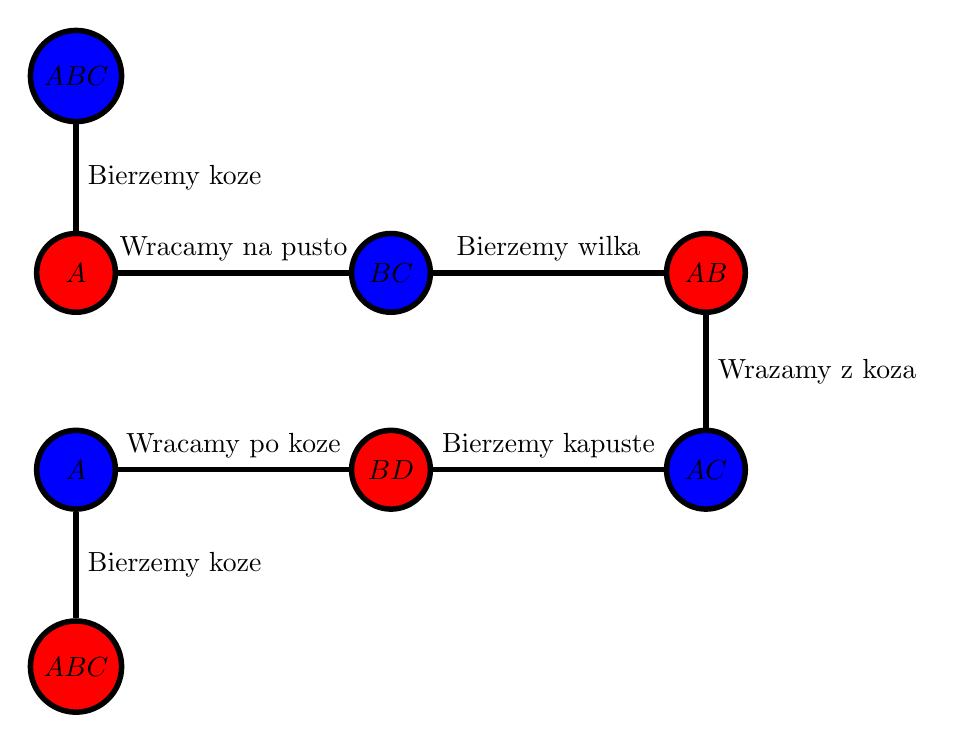
\begin{tikzpicture}[auto, node distance =2.5cm and 4cm, on grid, semithick, 
        state/.style={circle, top color=white, bottom color= processblue!20, draw, black, text=blue, 
        minimum width=1cm}, line width=0.7mm]
        \node[circle, fill=blue,draw=black, minimum width = 1cm] (ABCs) {$ABC$};
        \node[circle, fill=red, draw=black,minimum width = 1cm] (Af) [below=of ABCs] {$A$};
        \node[circle, fill=blue, draw=black,minimum width = 1cm] (BCs) [right=of Af] {$BC$};
        \node[circle, fill=red, draw=black,minimum width = 1cm] (ABf) [right=of BCs] {$AB$};
        \node[circle, fill=blue, draw=black,minimum width = 1cm] (ACs) [below=of ABf] {$AC$};
        \node[circle, fill=red, draw=black,minimum width = 1cm] (BCf) [left = of ACs] {$BD$}; 
        \node[circle, fill=blue, draw=black,minimum width = 1cm] (As) [left=of BCf] {$A$};
        \node[circle, fill=red, draw=black,minimum width = 1cm] (ABCf) [below=of As] {$ABC$};

        \path (ABCs) edge [] node[right] {Bierzemy koze} (Af);
        \path (Af) edge [] node[above] {Wracamy na pusto} (BCs);
        \path (BCs) edge [] node[above] {Bierzemy wilka} (ABf); 
        \path (ABf) edge [] node[right] {Wrazamy z koza} (ACs);
        \path (ACs) edge [] node[above] {Bierzemy kapuste} (BCf);
        \path (BCf) edge [] node[above] {Wracamy po koze} (As);
        \path (As) edge [] node[right] {Bierzemy koze} (ABCf);
\end{tikzpicture}


\end{center}

\end{solution}
\end{problem}


\begin{problem}{Rzedy automorfizmow}
    
Oblicz rzedy grup automorizmow grafu G:

\subproblem
\begin{center}
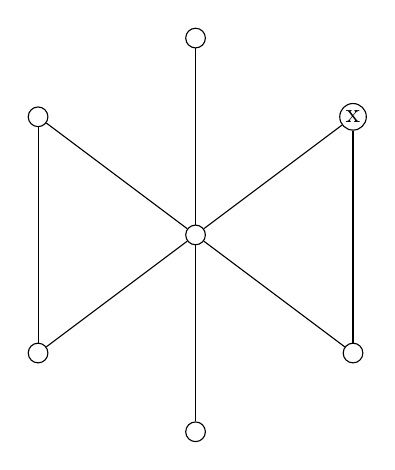
\begin{tikzpicture}[scale=1, every node/.style={circle, draw, inner sep=1pt, minimum size=0.25cm}]
    % Wierzchołki
    \node (center) at (0, 0) {};
    \node (top) at (0, 2.5) {};
    \node (bottom) at (0, -2.5) {};


    \node (topleft) at (-2, 1.5) {};
    \node (topright) at (2, 1.5) {x};
    \node (bottomleft) at (-2, -1.5) {};
    \node (bottomright) at (2, -1.5) {};
   

    % Krawędzie
    \draw (center) -- (top);
    \draw (center) -- (bottom);
    \draw (center) -- (topleft);
    \draw (center) -- (topright);
    \draw (center) -- (bottomleft);
    \draw (center) -- (bottomright);
    \draw (topleft) -- (bottomleft);
    \draw (topright) -- (bottomright);
\end{tikzpicture}
\end{center}

\subproblem
\begin{center}
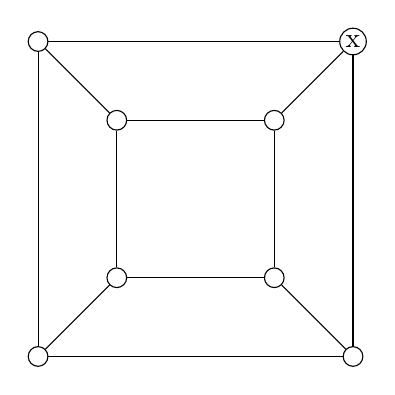
\begin{tikzpicture}[scale=1, every node/.style={circle, draw, inner sep=1pt, minimum size=0.25cm}]
    % Wierzchołki

    \node (topleft) at (-2, 2) {};
    \node (topright) at (2, 2) {x};
    \node (bottomleft) at (-2, -2) {};
    \node (bottomright) at (2, -2) {};
    \node (A) at (-1, 1) {};
    \node (B) at (1, 1) {};
    \node (C) at (-1, -1) {};
    \node (D) at (1, -1) {};

    % Krawędzie

    \draw (A) -- (B);
    \draw (B) -- (D);
    \draw (C) -- (A);
    \draw (D) -- (C);
    \draw (A) -- (topleft);
    \draw (B) -- (topright);
    \draw (C) -- (bottomleft);
    \draw (D) -- (bottomright);
    \draw (bottomright) -- (bottomleft);
    \draw (bottomright) -- (topright);
    \draw (topleft) -- (bottomleft);
    \draw (topright) -- (topleft);


\end{tikzpicture}
\end{center}

\end{problem}

\begin{problem}{Rzad automorfizmow grafu Petersona}

Oblicz rzad grupy automorizmow grafu G-Petersena.
    \begin{center}
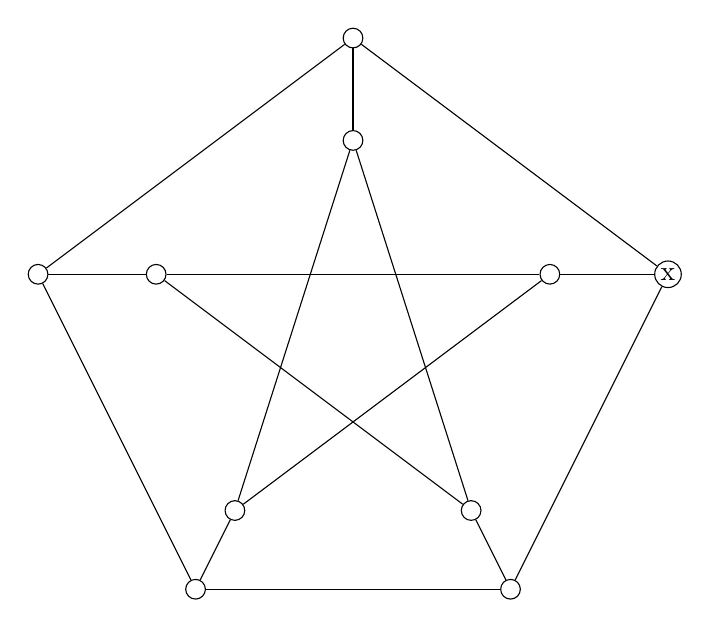
\begin{tikzpicture}[scale=1, every node/.style={circle, draw, inner sep=1pt, minimum size=0.25cm}]
    % Wierzchołki

    \node (top) at (0, 5) {};
    \node (topleft) at (-4, 2) {};
    \node (topright) at (4, 2) {x};
    \node (bottomleft) at (-2, -2) {};
    \node (bottomright) at (2, -2) {};
    \node (mtop) at (0, 3.7) {};
    \node (mtopright) at (2.5, 2) {};
    \node (mbottomright) at (1.5, -1) {};
    \node (mbottomleft) at (-1.5, -1) {};
    \node (mtopleft) at (-2.5, 2) {};
    % Krawędzie
    
    \draw (top) -- (topleft);
    \draw (topleft) -- (bottomleft);
    \draw (bottomleft) -- (bottomright);
    \draw (bottomright) --(topright);
    \draw (topright) -- (top);

    
    \draw (mtop) -- (mbottomleft);
    \draw (mtopleft) -- (mbottomright);
    \draw (mbottomleft) -- (mtopright);
    \draw (mbottomright) --(mtop);
    \draw (top) -- (mtop);
    \draw (mtopleft) -- (mtopright);

    \draw (topleft) -- (mtopleft);
    \draw (bottomleft) -- (mbottomleft);
    \draw (bottomright) --(mbottomright);
    \draw (topright) -- (mtopright);
    

\end{tikzpicture}
\end{center}

   

\end{problem}

\begin{problem}{Nieizomorficzne grafy z trzema i czterema wierzcholkami}
    Wykaz, ze z dokladnoscia do izomorfizmu:

    \subproblem Istnieja dokladnie cztery grafy z trzema wierzcholkami.
   
    \subproblem Istnieja dokladnie jedenascie grafow z czterema wierzcholkami.
    
\end{problem}

\begin{problem}{Nieizomorficzne grafy 3-regularne z 6 wierzcholkami}


\begin{solution}
    Mamy conajmniej dwie mozliwosci na rozwiazanie:
    
    \subproblem Wprost

    \subproblem Dwa grafy 3-regularne z 6 wierzcholkami sa nieizomorficzne iff ich dopelnienia sa nieizomorficzne z 6 wierzcholkami 2-regularne. $\leftarrow$ dowod chyba trzeba tego faktu.
    
\end{solution}
    
\end{problem}

\begin{problem}{k- wymiarowe kostki}
    
    Przez $Q_{k}$ oznaczmy graf k-wymiarowej kostki. tj. wierzcholkami w $Q_{k}$ sa wszystkie k-elementowe ciagi zer i jedynek. oraz dwa wierzcholki sa sasiednie wtedy i tylko wtedy, kiedy odpowiadajace im ciagi roznia sie dokladnie jedna wspolrzedna.

    \subproblem Wykaz, ze $n(Q_{k}) = 2^{k}$.

    \subproblem Wykaz, ze $m(Q_{k}) = k2^{k-1}$.

    \subproblem Udowodnij, ze $Q_{k}$ jest grafem dwudzielnym.

    \begin{solution}
        
    \end{solution}
\end{problem}

\begin{problem}{Ogolne wlasnosci grafu}
    Niech $V = \left\{ 1,2,\dot, n \right\}$. Okresl liczbe nieidentycznych
    
    \subproblem grafow prostych o zbiorze wierzcholkow w $V$

    \subproblem grafow o zbiorze wierzcholkow $V$ i m krawedziach, jesli dopuszczamy petle i krawedzie wielokrotne

    \subproblem digrafow jak w poprzednim podpunkcie

    \begin{solution}
        
    \end{solution}

\end{problem}

\begin{problem}{Liczba krawedzi w grafie dwudzielnym}

    Udowodnij, ze w grafie dwudzielnym o n wierzcholkach, liczba krawedzi jest rowna conajwyzej $\lfloor \tfrac{n^{2}}{2} \rfloor$.
    
    \begin{solution}
        
    \end{solution}
\end{problem}
\end{document}
